\subsection{Mediator}
\label{mediator}

\textbf{Scopo}: Comportamentale \\
\textbf{Raggio d'azione}: Oggetti

\paragraph{Definizione} Il pattern Mediator definisce un oggetto che incapsula il modo in cui un insieme di oggetti interagisce. Il mediatore promuove l’accoppiamento libero impedendo agli oggetti di riferirsi esplicitamente tra loro e consente di variare la loro interazione in modo indipendente.

\paragraph{Nota} È bene notare che la POO incoraggia la distribuzione di comportamento tra gli oggetti, portando ad una struttura con molte connesioni tra oggetti. Le molte interconnessioni rendono meno probabile che un oggetto possa funzionare senza il supporto di altri.

\begin{figure}[H]
    \centering
    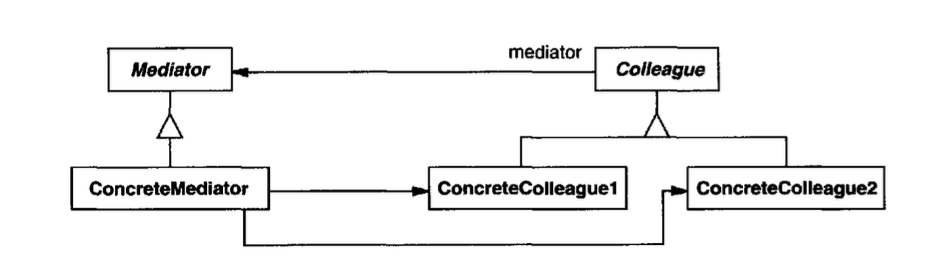
\includegraphics[width=0.8\linewidth]{assets/pattern/mediator/mediator-struttura.png}
    \caption{Class Diagram del pattern Mediator}
\end{figure}

\paragraph{Struttura e Conseguenze} 
\begin{itemize}
    \item \textbf{Mediator}: definisce un’interfaccia che espone i metodi che abilitano la comunicazione tra i componenti in relazione o agisce come punto centrale per la gestione delle interazioni tra i vari partecipanti. Il Mediatore conosce e mantiene i riferimenti agli oggetti dei partecipanti e facilita la loro comunicazione. Gestisce le dipendenze e incapsula il comportamento.
    \item \textbf{ConcreteMediator}: implementa l’interfaccia Mediator e, nel definire i metodi dell’interfaccia, realizza uno specifico comportamento di cooperazione tra i componenti. Gestisce effettivamente la comunicazione tra i partecipanti, implementando i metodi definiti nell'interfaccia del Mediatore. Essa conosce i partecipanti e regola il flusso delle comunicazioni tra di essi.
    \item \textbf{Colleague}: definisce l’interfaccia che rappresenta un componente del sistema che deve comunicare tramite il Mediatore. Ogni Colleague conosce solo il Mediatore e non ha una conoscenza diretta degli altri Colleague. Essi inviano e ricevono messaggi tramite il Mediatore.
    \item \textbf{ConcreteColleague}: classe concreta che implementa l'interfaccia dei Colleague. Ogni ConcreteColleague è un componente specifico del sistema che deve comunicare con gli altri Colleague tramite il Mediatore.
\end{itemize}

Il pattern mediator permette di limitare la sottoclasse del comportamento, separare i colleghi, semplificare i protocolli degli oggetti, facilitare l’aggiunta di nuovi componenti, astrarre la cooperazione tra oggetti, favorire il riutilizzo dei Mediator e centralizzare il controllo delle interazioni.

\begin{figure}[H]
    \centering
    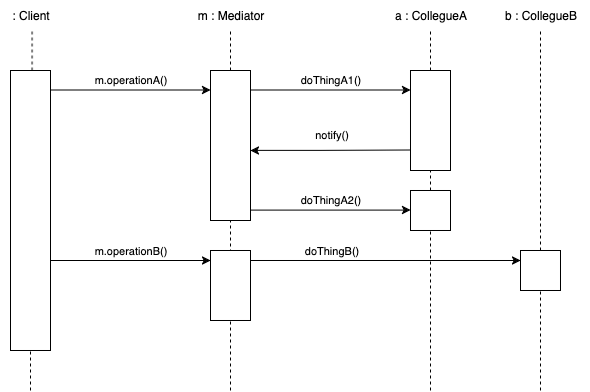
\includegraphics[width=0.8\linewidth]{assets/pattern/mediator/mediator-sequence.drawio.png}
    \caption{Sequence Diagram del pattern Mediator}
\end{figure}

\paragraph{Pattern correlati}
\begin{itemize}
    \item \textbf{Observer} (\ref{observer})
    \item \textbf{Facade} (\ref{facade})
    \item \textbf{Command} (\ref{command})
    \item \textbf{Chain of Responsibility} (\ref{chain-of-responsability})
    \item \textbf{Strategy} (\ref{strategy})
\end{itemize}

\newpage